
\section{Introduction}
Reading is an intricate task involving multiple processes located in different areas in the brain \citep{price2012review}. Errors in reading can result from dyslexia, a disorder involving a variety of such errors. Dyslexia is a highly common disorder with estimates of prevalence ranging from 5\% to 17.5\% \citep{ss05}, pointing to the need for accurate and accessible diagnosis. However, current diagnostic procedures require experts, and are mostly lengthy and expensive. In this study, we aim to provide an accessible, reliable and cheap diagnosis tool for dyslexia. We do this by showing that rich probabilistic graphical models can diagnose dyslexia closely to how experts do, rendering them accurate, reliable and automated tool for diagnosis. Moreover, by providing probability distributions of errors given target words in screening tests, models can be used for future improvement of the diagnosis procedure and understanding of dyslexia. Finally, our results provide a novel and quantitative perspective on an ongoing debate regarding the nature of dyslexia (e.g., \citealp{eg14}).

A dyslexic person may read the word {\it three} as 'there', as 'tree' or as 'four'. Despite this heterogeneity, many studies in the field of reading disorders focus on measures of speed and accuracy to characterize dyslexia, thus possibly ignoring the rich structure of types of reading errors. These studies often assume a common phonological \citep{r14, rrddcw03, s98, s01} or sensorimotor \citep{s01} cause to all reading errors. However, an alternative approach views dyslexia as an umbrella term for various deficiencies, or dyslexia subtypes, each characterized by specific error types (e.g., \citealp{mn73, ellis2013human, ck12, friedmann2016types}). According to this approach, each of the errors in the example above could result from a different subtype of dyslexia. This approach suggests that fundamental aspects of reading disorders lay in the complex structure of reading errors.

We explore the structure of reading errors and the heterogeneity of dyslexia using probabilistic tools. Probabilistic graphical models have several advantages as a framework for modelling reading errors. Probabilistic models allow explicitly capturing a dependency structure among variables in the problem, making learning more efficient. Probabilistic graphical models provide both diagnoses and explicit error distributions per each type of dyslexia and target word, as learned from the corpus data, and can naturally follow an error-generation process.

We use two families of graphical models. First, we construct Na\"{\i}ve Bayes models which are well-known for having a good performance as classifiers with relatively low model complexity (see, e.g., \citealp{lit92}). These models are thus suitable for the classification of reading errors. Next, we construct a Latent Dirichlet Allocation based (LDA-based) model, which has been proven to well capture generation processes in the context of writing and text \citep{bnj03, rgss04}. In such a model, the generation of reading errors made by a dyslexic person is a more complex process than that in a Na\"{\i}ve Bayes model, as it assumes that errors are generated according to a mixture of subtypes of dyslexia. An LDA model is therefore a natural candidate for dyslexia analysis.

We compare the models on two different tasks. First, we identify the probabilistic model that best performs on the task of diagnosing dyslexia. We achieve this by comparing the diagnoses of the models to those of experts. Secondly, we explore which model best captures the complex structure of the patterns of reading errors. We achieve this by comparing the models on the task of predicting unseen errors. Finally, the performance of the models is used to explore the question of whether reading errors do result from different subtypes of dyslexia, or rather from one general malfunction.

The rest of the chapter is organized as follows: section 1.2 describes the related literature of probabilistic graphical models and of dyslexia. It also provides a summary of the major views of dyslexia in the current literature of reading disorders. Section 1.3 describes the structure and size of the data that was used in this study. Section 1.4 provides a detailed description of the probabilistic graphical models. Finally, section 1.5 describes the results of this study: the performance of the models on the task of diagnosing dyslexia (section 1.5.1), and the performance of the models in predicting reading errors (section 1.5.2).


\section{Related work}
\subsection{Probabilistic graphical models}
The LDA model was introduced a decade ago to discover topics in documents, and has been most influential since. Three main algorithms for approximate inference in the model were proposed: Variational Expectation-Maximization \citep{bnj03}, the Expectation-Propagation \citep{ml02}, and Collapsed Gibbs Sampling \citep{gs04}. In this chapter we use the latter method. The generative process described by the LDA model commences in Dirichlet priors which are often chosen to be uniform. However, following the demonstration of the importance of using non-uniform priors for this model \citep{wmm09}, we use these and not uniform priors in this study.

\subsection{Dyslexia and reading errors}
Literature on reading disorders presents various accounts of the causes of developmental dyslexia. One central approach describes developmental dyslexia as a disorder that can be reduced into a single cause, and will be referred to hereby as the {\it single-type} approach. The most influential example of this approach is the {\it phonological deficit hypothesis}. According to this theory, developmental dyslexia originates from a deficit affecting either the representations and processing of speech sounds \citep{ss05, s00, s98}, or as other authors have argued, from the access to these representations \citep{rs08}. This hypothesis had influence on much research in neuroscience and brain imaging studies (e.g., \citealp{bdvsgmg13, d09, vgpsh13, grggvfb02, r14, rrddcw03}).

Another central approach describes dyslexia as a heterogeneous disorder, having several different causes, and will be referred to hereby as the {\it subtypes} approach. The most influential example of this approach derives from the {\it Dual-Route Reading Model} \citep{cc93, ck12, mn73}, describing the process of reading by several processing stages and routes (General Introduction figure 1). According to this approach, there are subtypes of dyslexia, each resulting from a deficit or malfunction in a different stage in the process of reading. For example, reading {\it signs} as 'sings' may result from a specific malfunction in letter position processing during the early visual-orthographic stage, and is in this case ascribed to Letter Position Dyslexia \citep{fg01}. However, reading {\it signs} while pronouncing the 'g', may be caused by Surface Dyslexia, characterized by reading irregular words according to the regular grapheme-to-phoneme conversion rules \citep{c83}. The deficit leading to Surface Dyslexia occurs in one of two long-term memory lexicons, the orthographic or phonological lexicon, or in the information processing between them. Brain imaging studies following this approach aim to identify the neural correlates of different subtypes of dyslexia {e.g., \citealp{jct03, lptbadc09}). It is important to note, that while the single-type approach refers to developmental dyslexia, the subtype approach refers to both developmental and acquired (i.e., following a brain damage) dyslexias.

The single-type approach and the subtypes approach use different procedures to diagnose dyslexia. The diagnostic procedure based on the single-type approach mainly uses phonological tasks, for example, asking the subject to swap between the first phonemes in the two auditorily presented words {\it fresh bread} (expecting to get 'bresh fread'). When otherwise using reading tasks, the degree of dyslexia is assessed by measuring general accuracy and speed in such tasks, while disregarding the types of errors which were made. However, the diagnostic procedure based on the subtypes approach mainly uses reading tasks, asking the subject to read aloud a list of words that are prone to erroneous reading. These tests assess the subtype of dyslexia by counting the errors made of each type. 

Another group of studies aim to characterize dyslexia subtypes (e.g., \citealp{p06}), however the diagnostic procedure in these studies is not based on data of error types in reading tests, but on measures of speed and accuracy in various tasks. Several such studies have proposed probabilistic models to analyze the data (e.g., \citealp{plljbrak12}). See also \citet{rp14} for analysis of reading aloud data, however in contrast to our study, they were not concerned with error types in reading tests but focused on reading of nonwords by normal subjects.

\section{The data}
We test our models using reading tests collected from 313 Hebrew-speaking individuals with developmental dyslexia, aged 7 to 62 years, all tested and analyzed in the Language and Brain laboratory in Tel-Aviv University. Out of the 313 subjects, 97 were diagnosed with an Attention Deficit Disorder (ADD) in addition to dyslexia. This is, to our knowledge, the largest reading-errors corpus used so far (see \citealp{p07, rbl14}). The battery of tests has two parts: (1) screening-tests: reading tests given for initial assessment of dyslexia (TILTAN battery, \citealp{fg03}), and (2) varying post-tests which are determined according to the results of the screening-tests. These are used to further specify the diagnosis. Since different subjects take different post-tests, only the corpus of the screening tests was used in this study.

The screening test is composed of 196 target words in Hebrew, which are prone to erroneous readings. The audio responses of subjects are recorded, and then encoded before used in the model. Responses were encoded by experts in dyslexia diagnosis and research, into one of 19 different error types (table 1.1). Each of the 313 subjects therefore read 196 words in the screening-test, resulting in a corpus consisting of a total of 61,348 pairs of target-word and response.

\begin{table}

\centering
\begin{tabular}{|c|c|c|} \hline

& Error type & Dyslexia type\\
\hline
1 & Correct response & NS\\
2 & Consonant migration & LPD, VD\\
3 & Consonant omission & VD\\
4 & Consonant addition & VD\\
5 & Consonant substitution & VD\\
6 & Vowel migration & VLD, LPD, VD\\
7 & Vowel omission & VLD, VD\\
8 & Vowel addition & VLD, VD\\
9 & Vowel substitution & VLD, VD\\
10 & Semantic error & Other\\
11 & Morphological error & Other\\
12 & Surface error & SD\\
13 & Visual error (left side) & ND, VD\\
14 & Function word error & Other\\
15 & Letter doubling, or double omission & LPD, VD\\
16 & Attentional omission & AD\\
17 & Attentional vowel letter error & AD, VLD\\
18 & Attentional migration between words & AD\\
19 & Migration of end letters & VD\\

\hline\end{tabular}
\bigskip
\caption{List of error types and the possible responsible dyslexia types. NS - Normal State; LPD - Letter Position Dyslexia; VD - Visual Dyslexia; VLD - Vowel Letter Dyslexia; AD - Attentional Dyslexia; ND - Neglect Dyslexia; Other - Other types of dyslexia, such as phonological output buffer dyslexia or deep dyslexia, which are diagnosed based on additional post-tests.}
\end{table}

Based on the screening tests and on additional post-tests, had these been conducted, each subject is diagnosed by an expert by marking the subtypes of dyslexia that he or she has. We represent each diagnosis as a multi-label binary vector of length 7, corresponding to seven dyslexia subtypes: 'Letter position dyslexia', 'Attentional dyslexia', 'Neglexia', 'Surface dyslexia', 'Visual dyslexia', 'Vowel letter dyslexia' and 'Normal state'.

The collected data corpus is in Hebrew, therefore it is important to discuss the applicability of this work to other languages, specifically English. The underspecification of vowels in Hebrew makes the Hebrew orthography neighborhood denser than that of languages such as English. An example of this is that in Hebrew, letter transpositions inside a word are more likely to result in another existing word, than in English. This property makes some dyslexias more easily detectable in Hebrew than in English. However, once the relevant stimuli are selected for an English reading task, the same dyslexias with the same properties are detectable in both languages. And indeed, the dyslexias we describe have all been identified in English (For a comprehensive survey of this literature of dyslexia types in English, see for example \citealp{ck12}; for the specific dyslexias that we describe here see Letter position dyslexia: \citealp{kohnen2012slime}; Attentional dyslexia: \citealp{sc98, sw77}; Neglexia: \citealp{vba10}; vowel dyslexia: \citealp{kf11}; Surface dyslexia: \citealp{bd95, cbc06, cc93, c83}). Similarly, dyslexia subtypes have been identified also in Arabic \citep{friedmann2012letter, friedmann2014types}, and in Italian (e.g., \citealp{job1984developmental}. This work can therefore be expanded to English and other languages.

\section{The models}
Bayesian models are expressive statistical models. Typically, these are used for mathematically modeling assumptions regarding the manner in which data (in this case, reading errors), is generated. We construct three different probabilistic graphical models for this purpose: a Latent Dirichlet Allocation (LDA) model, and two Na\"{\i}ve Bayes models.

\begin{figure*}
\vspace{.3in}
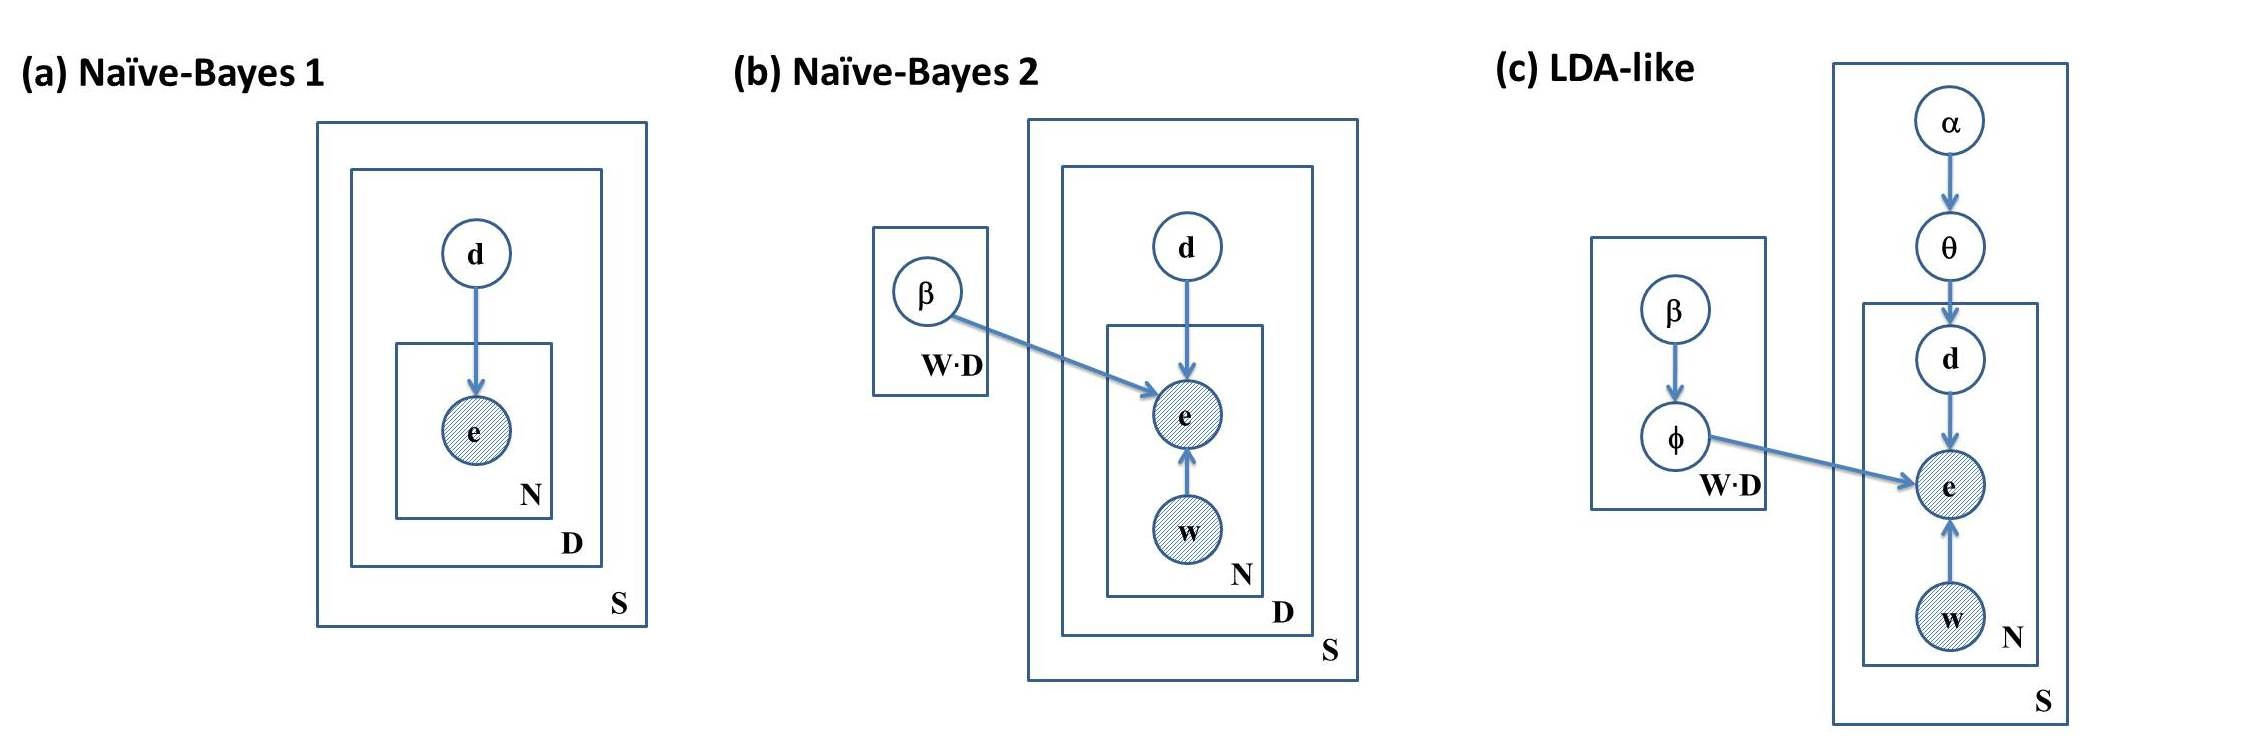
\includegraphics[width=\textwidth]{Figures/Ch1/figure_graphical_models}
\caption{Plate diagrams for all three models. (a) Na\"{\i}ve-Bayes 1 (b) Na\"{\i}ve-Bayes 2 (c) LDA-like model. $S$ represents the total number of subjects, $N$ the number of target-words in the screening test, $W$ the size of the vocabulary of the target-words, and $D$ represents the total number of dyslexia states. $e$ represents an error type, $w$ a target-word and $d$ a dyslexia state. In the LDA model, $\theta$ represents a diagnosis, $\phi$ represents a word-error-dyslexia distribution. $\alpha$ and $\beta$ are the Dirichlet priors for these distributions respectively.}
\end{figure*}

\subsection{Na\"{\i}ve Bayes models}
We begin to explore the generation process of reading errors with the class of Na\"{\i}ve Bayes models. Na\"{\i}ve Bayes models have shown much success in classification tasks, and could therefore fit the task of classifying reading error into dyslexia subtypes. 

The types of the errors made by the subjects are denoted in the models by $ e_i (i = 1, \dots , N) $. This variable takes one of $E$ possible values $ e_i \in {1, \dots , E} $, where $E$ stands for the number of possible error-types including a correct response. Another observed variable of the model represents the target-words. We denote it by $ w_i (i = 1, \dots , N) $, where $N$ represents the number of target-words in the screening-test. This variable can have one of $W$ possible values $ w_i \in {1, \dots , W} $. Since in our case each target-word is present only once in the screening-test, we have $ W = N $.

In all three models, a {\it dyslexia state} defines a hidden variable that stands for a state associated with a specific subtype of dyslexia, and is characterized by particular reading errors. For example, being in a state of low orthographic within-word attention could be associated with Letter Position Dyslexia (LPD), typically leading to letter migration errors. We denote a dyslexia state by $d_i$, where $d_i$ can have one of D $ d_i \in {1, \dots ,D} $ dyslexia states. We have 7 such states as described above.

In all models, $S$ stands for the total number of subjects, $N$ stands for the number of target-words in the screening test, $W$ is the size of the vocabulary of the target-words, and $D$ stands for the total number of dyslexia states. $e$ represents an error type, $w$ a target-word and $d$ a dyslexia state.

\subsubsection{Word independent Na\"{\i}ve Bayes Model}
Typically, clinicians use the screening test to diagnose dys\-lexic subjects based on the total counts of different errors types they make. This approach disregards the specific target-words on which the errors were made, for instance, whether it is a word that many subjects misread, or specific subjects only. This diagnosis procedure can be modeled with a Na\"{\i}ve-Bayes model in which the probability of an error-type depends on the dyslexia subtype only. In what follows, we refer to this model as the Na\"{\i}ve Bayes 1 (NB1) model.

\paragraph{Model description}
For test results of a single subject, the joint distribution of the NB1 model factorizes as:
\[ p(\bar{e}, \bar{w}, d) = p(d) \prod_{i=1}^N p(e_i \mid d) p(w_i), \]
where the subscript $ i $ runs over all word-error pairs in the screening-test. Note that each error is independent of the specific target-word on which it was made. Figure 1.1a describes the plate diagram of the model.

\subsubsection{Word dependent Na\"{\i}ve Bayes Model}
A more complex model is a Na\"{\i}ve Bayes model in which the probability of an error is dependent on the dyslexia subtype and also on the target-word. We examine this model as well and will refer to it in what follows as the Na\"{\i}ve Bayes 2 (NB2) model.

\paragraph{Model description}
In this model the response of the subject $ e_i $ is dependent on the $ i^{th} $ target-word $ w_i $ and on the dyslexia state $ d_i $. Similarly to the NB1 model, the joint distribution for the NB2 factorizes as:
\[ p(\bar{e}, \bar{w}, d ; \beta) = p(d) \prod_{i=1}^N p(e_i \mid d, w_i ; \beta) p(w_i), \]
where the subscript $i$ runs over all word-error pairs in the screening-test as before. Figure 1.1b describes the plate diagram of the model.

\subsection{The LDA model}
We continue our inquiry with a particular family of Bayesian models that has attracted much attention in the past decade, the Latent Dirichlet Allocation (LDA) Model \citep{bnj03}. The LDA model enables inferring unobserved variables given observed data, and has shown much success in capturing generative processes of text documents \citep{bnj03, rgss04}.

\subsubsection{Model description}
The LDA model captures the case where a person can suffer from a mixture of different dyslexia subtypes. According to this model, each person has a unique distribution over dyslexia subtypes. Additionally, each dys\-lexia subtype has a unique distribution of expected errors for a given target-word. When a person reads a target-word, a particular dyslexia subtype is directing the way by which the word is read. The response then dependents both on the dyslexia subtype and the target-word. We therefore define two additional hidden variables: (1) A {\it diagnosis} $ \theta_{s} $, which is a distribution over dyslexia states $ d_i $ for a subject, learned from the data; (2) A {\it word-error-dyslexia distribution} $ \phi_{wed} = p(e_i = e \mid w_i = w , d_i= d) $, which is a distribution for all subjects in which, given a dyslexia state $d$ and a target-word $w$, each error has a certain probability of occurring. For example, given an LPD state, and the target-word {\it three}, the erroneous response {\it there} would be of high probability, but {\it tree} would be of a lower one. Similarly, given a normal state, and the target-word {\it three}, all error responses would have low probabilities except for the (correct) response {\it three}. 

The input to the model is the word-error pairs of all subjects. The hidden variables discovered by the model are: (1) $N$ dyslexia states for each subject; (2) The diagnosis of each subject - $ \theta_{s} $; and (3) A single word-error-dyslexia distribution $ \phi_{wed} $ for all subjects. Figure 1.1c describes the plate diagram of the dyslexia-state model.

\subsubsection{Dirichlet priors}
The generative process we use to model reading errors uses two Dirichlet priors from which the two distributions $ \theta_{s}$, $\phi_{wed} $ are sampled. Dirichlet priors are often chosen to be uniform. However, adding priors that adequately describe the generative process could enhance model performance. As the subtype approach to dyslexia has developed ways to detect typical reading errors for each dyslexia subtype, this prior knowledge can be incorporated into the LDA model. We tested the model both with this prior knowledge coded into it and without it.

The expert knowledge is used for sampling the word-error-dyslexia distribution and we denote it by $ \beta_{wed} $. This knowledge tells us about the error expected for each target-word given a dyslexia state (figure 1.1c). For example, given an LPD dyslexia-state, the word {\it three} is more likely to be read as {\it there} than {\it tree} or {\it four}. We incorporate this into the model by assigning a higher prior value $ \beta_{high} $ to the more probable responses of an LPD dyslexia-state, in this example {\it there}. We also assign a lower prior value $ \beta_{low} $ to the less probable responses, in this case {\it tree} and {\it four}. This is repeated for all dyslexia-states, including the normal state.

\subsubsection{Parameter estimation}
Gibbs sampling is a form of a Markov Chain Monte Carlo (MCMC) method which is widely used for parameter estimation in topic models \citep{gs04, rgss04}. We use Gibbs sampling to construct a Markov chain between dyslexia-states, where the order of the Markov chain is based on the order of target-words in the reading-test. In each step, a dyslexia-state is sampled from its posterior distribution conditioned on all other variables in the model (see derivation below): 

\begin{equation}
\begin{split}
p(d_i = d\mid w_i = w, e_i = e, d_{-i}, w_{-i}, e_{-i}, \alpha, \beta) \propto \\
\frac{ C_{wed, -i} + \beta_{wed} } {\sum_{e'} [C_{we'd, -i} + \beta_{we'd}] } \frac{ C_{ds, -i} + \alpha_{ds} } {{\sum_{d'}[ C_{d's, -i} + \alpha_{d's}] }},
\end{split}
\end{equation}

where $ d_i=d $ represents the assignment of the $ i^{th} $ word-error pair to dyslexia-state $d$. $ w_i = w $ represents the observation that the $i^{th}$ target-word is $w$, and $e_i = e $ represents the observation that the $i^{th}$ error type is $e$. $ d_{-i} $ represents all dyslexia-state assignments excluding the current $i^{th}$ instant. $ w_{-i} $ represents all target-words observations excluding the current $i^{th}$ instant. Similarly, $ e_{-i} $ represents all target-words observations excluding the current $i^{th}$ instant.
$ C_{wed, -i} $ represents the number of times the word-error pair ($w, e$) was assigned to the dyslexia-state $d$, excluding the current instance. $ C_{ds, -i} $ represents the number of times the dyslexia-state $d$ was assigned to the dyslexic person $s$. $ \alpha_{ds} , \beta_{wed} $ are the Dirichlet prior weights (see 4.1.2).
At each step of the Markov chain, we update the diagnoses of the subjects $ { \{ \theta_{s} \} }_{s=1}^S $ and the word-error-dyslexia distribution $ \phi_{wed} $ according to the dyslexia-state assignments $ \bar{d_{s}} $. These are then used to assess the accuracy and predictive power of the model.

We describe the derivation of the update rule (Eq. 1.1) following similar lines to those in \citet{gs04}, with the modifications required for our dyslexia-model (figure 1.1C):

The joint distribution of the model is given by:

\begin{equation*}
\begin{split}
&p(\bar{e},\bar{w},\bar{d},\Theta,\Phi;\alpha,\beta) = \\
&p(\Phi\mid\beta)p(\beta)\prod_{s = 1}^S p(\bar{e}_s\mid\bar{d}_s, \bar{w}_s) p(\bar{w}_s)p(\bar{d}_s\mid\Theta_s)\\ &p(\Theta_s\mid\alpha_s)p(\alpha_s) = \\
&p(\Phi\mid\beta) p(\beta) \prod_{s = 1}^S \prod_{i=1}^N p(e_{i, s} \mid w_{i, s}, d_{i, s}) p(d_{i, s}\mid\Theta_s) p(\Theta_s\mid\alpha_s)\\
&p(w_{i, s}) p(\alpha_s).
\end{split}
\end{equation*}

Given that $p(\Theta_s\mid\alpha_s)$ and $p(\Phi\mid\beta)$ are Dirichlet priors, and that $p(w_{i, s})$ are constant, rewriting the expression for the joint distribution, we get:

\begin{equation*}
\begin{split}
&p(\bar{e}, \bar{w}, \bar{d}, \Theta, \Phi; \alpha, \beta) \propto \\
&\prod_{s=1}^S \prod_{w=1}^W \prod_{e=1}^E \prod_{d = 1}^D \phi_{wed}^{C_{wed} + \beta_{wed} - 1} \theta_{ds}^{C_{ds} + \alpha_{ds} - 1}.
\end{split}
\end{equation*}

Integrating out $\theta$ and $\phi$, we get:

\begin{equation*}
\begin{split}
&p(\bar{e},\bar{w},\bar{d};\alpha,\beta) \propto \\
&\iint \prod_{s=1}^S \prod_{w=1}^W \prod_{e=1}^E \prod_{d = 1}^D  \phi_{wed}^{C_{wed} + \beta_{wed} - 1} \theta_{ds}^{C_{ds} + \alpha_{ds} - 1} \mathrm{d}\theta \mathrm{d}\phi = \\
&\int \prod_{s=1} \theta_{ds}^{C_{ds} + \alpha_{ds} - 1} \mathrm{d}\theta \prod_{w=1}^W \prod_{d = 1}^D \int\prod_{e=1}^E \phi_{wed}^{C_{wed} + \beta_{wed} - 1} \mathrm{d}\phi = \\
&\frac{\prod_{d = 1}^D\Gamma(C_{ds} + \alpha_{ds})}{\Gamma(\sum_{d' = 1}^D (C_{d's} + \alpha_{d's}))}\prod_{w=1}^W\prod_{d = 1}^D \frac{\prod_{e = 1}^E\Gamma(C_{wed} + \beta_{wed})}{\Gamma(\sum_{e' = 1}^E (C_{we'd} + \beta_{we'd}))}.
\end{split}
\end{equation*}

The posterior distribution for the $i^{th}$ dyslexic state can now be expressed using the expression for the joint distribution:

\begin{equation*}
\begin{split}
&p(d_i=d\mid w_i=w, e_i=e, d_{-i}, w_{-i}, e_{-i}; \alpha, \beta) \propto \\
&\frac{p(\bar{e},\bar{w},\bar{d};\alpha,\beta)}{p(\bar{e}_{-i},\bar{w}_{-i},\bar{d}_{-i};\alpha,\beta)}.
\end{split}
\end{equation*}

The numerator and denominator of the above fraction, differ only by the counts having the $i^{th}$ pair of word-error in them, whereas all other terms cancel out. The posterior distribution thus results as the above update rule (Eq. 1.1).

\section{Experiments}
We conduct two experiments with the data. In the first, described in section 1.5.2, we compare three graphical models to find which model most accurately predicts dyslexia diagnosis. In principle, this model can be used to automate dyslexia diagnosis. In the second experiment, described in section 1.5.3, we compare the quality by which these three graphical models predict specific reading errors. The best model to predict errors could contribute to the better characterization of dyslexia.

\subsection{Experimental set-up}
We use two different types of cross validation, first leaving out a set of subjects and then leaving out a set of word readings of the test subjects. Specifically, we randomly split the data into a training-set with 219 subjects (70\%) and a test-set with 94 subjects (30\%), controlled to have the same proportion of subjects who are also diagnosed with Attention Deficit Disorder. See illustration in figure 1.2. The test-set is further divided into two equal-sized sets: a {\textit {\textbf {diagnosis-set}} with 98 pairs of target-words and subject responses, used to infer the diagnosis of test subjects, and a {\textit {\textbf {prediction-set}} also with 98 word-response pairs, used for assessing the predictions of the models. 

\begin{figure}[H]
\vspace{.3in}
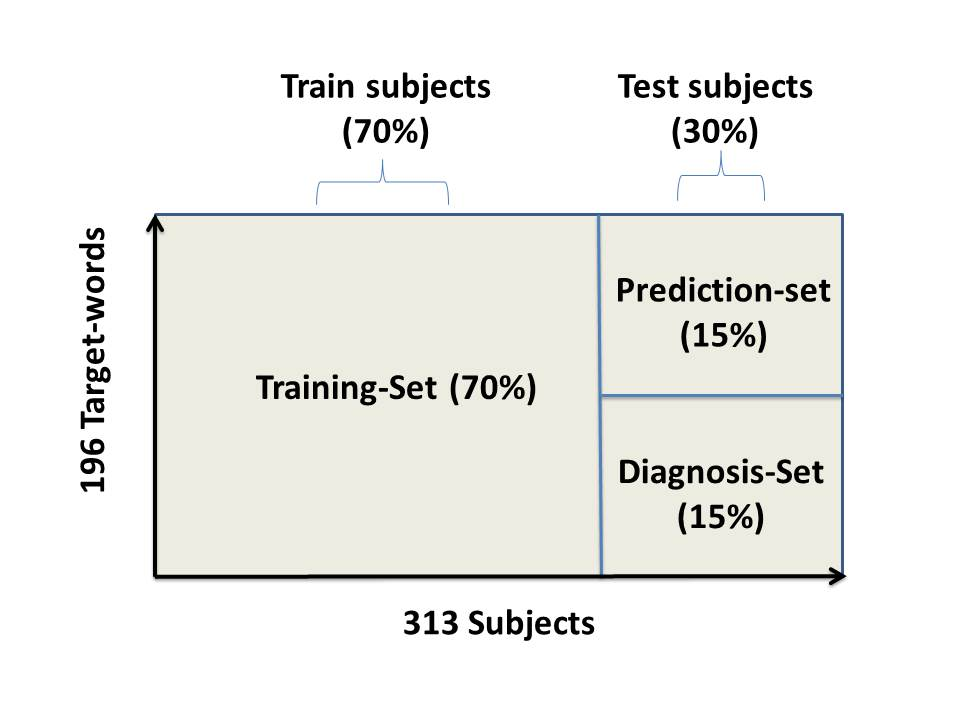
\includegraphics[width=\linewidth]{Figures/Ch1/trainTest2}
\caption{Data is partitioned into 3 sets. The dataset is first divided into a \textit {\textbf {training-set}} which contains reading-tests of 70\% of the subjects, and a test-set which contains the remaining 30\% of the data. The test-set is further divided into two subsets, a \textit {\textbf {diagnosis-set}} containing the first halves of the reading-tests, and a \textit {\textbf {prediction-set}} containing the remaining reading-tests of the test subjects.}
\end{figure}

\subsection{Probabilistic modeling as a dyslexia diagnosis tool}
Automation of the diagnosis process could facilitate the accessibility of the process to many people and increase awareness to treatment of specific reading deficits. We compare the automatic diagnosis of the three models -- NB1, NB2 and LDA -- to those given by experts, to test if the automated tool can indicate the diagnosed dyslexia type with high accordance to diagnoses given by experts.
We evaluate the diagnosis quality as follows. The automatic diagnosis is based on the diagnosis-set. This set is used to infer the diagnosis distribution $ \theta_{s} $ for each subject. The accuracy of the models is then assessed using the diagnoses given by experts. The prediction-set together with the diagnosis distribution $ \theta_{s} $ are later used for the evaluation of the predictive power of the models. The prediction-set is therefore not used in the diagnosis process.
Diagnosis quality of the two Na\"{\i}ve Bayes models, is estimated by computing 

\begin{equation}
p(d \mid \bar{e}) \propto p(d) \prod_{i = 1}^N [p(e_i \mid d)]^{C_{e_i}},
\end{equation}

\begin{equation}
p(d \mid \bar{e}, \bar{w}) \propto p(d) \prod_{i = 1}^N p(e_i \mid d, w_i),
\end{equation}

where the dyslexia prior $ p(d) $, the probability of error given a dyslexia subtype $ p(e_i |d) $, and the probability of an error given a dyslexia-type and a target-word $ p(e_i \mid d,w_i ) $ are estimated from the training group.

For the LDA model, we train the model on the training-set together with the diagnosis-set. The model is initialized with random dyslexia state assignments $ { \{ \bar{d}_{s} \} }_{s=1}^P $ which are then iteratively sampled according to the sampling rule in $(1)$. At each step of this process, we update the dyslexia distribution per each subject $ \theta_{s} $ and the word-error-dyslexia distribution $ \phi_{wed} $ according to the new sampled dyslexia-state.

The reason we train the model on the training-set and the diagnosis-set together is to avoid a discrepancy between the hidden dyslexia-states of the word-error-dyslexia distribution $ \phi_{wed} $, learned from the training-set, and those of the dyslexia distributions $ { \{ \theta_{s} \} }_{s \in test-set} $, learned from the diagnosis set. If the model is trained on the sets separately, the hidden states of these distributions might differ by a permutation relation. All results below are averages over 5 splits of subjects to train- and test- sets (allocations of subjects), and also over 10 different random initializations of the dyslexia state assignments (a total of 50 runs). 500 iterations were found to suffice for convergence (figure 1.4A).

We compare the diagnoses given by the three models to those given by experts. The Na\"{\i}ve-Bayes models are known to be strong classifiers and were designed by similar assumptions and guidelines to the ones held by diagnosticians, and therefore their diagnoses are expected to strongly correlate with those given by experts. The LDA model is designed to capture the generative process of the patterns of reading errors, (see section 1.5.2) but may therefore be a worse predictor of dyslexia subtypes. 
Note also that the diagnoses of the clinicians are given according to the results of the entire screening-tests and the post-tests results, whereas the diagnoses of the models are based on only halves of the screening-tests. This is expected to lower the maximum accuracy for all models.

\begin{figure}[H]
\vspace{.3in}
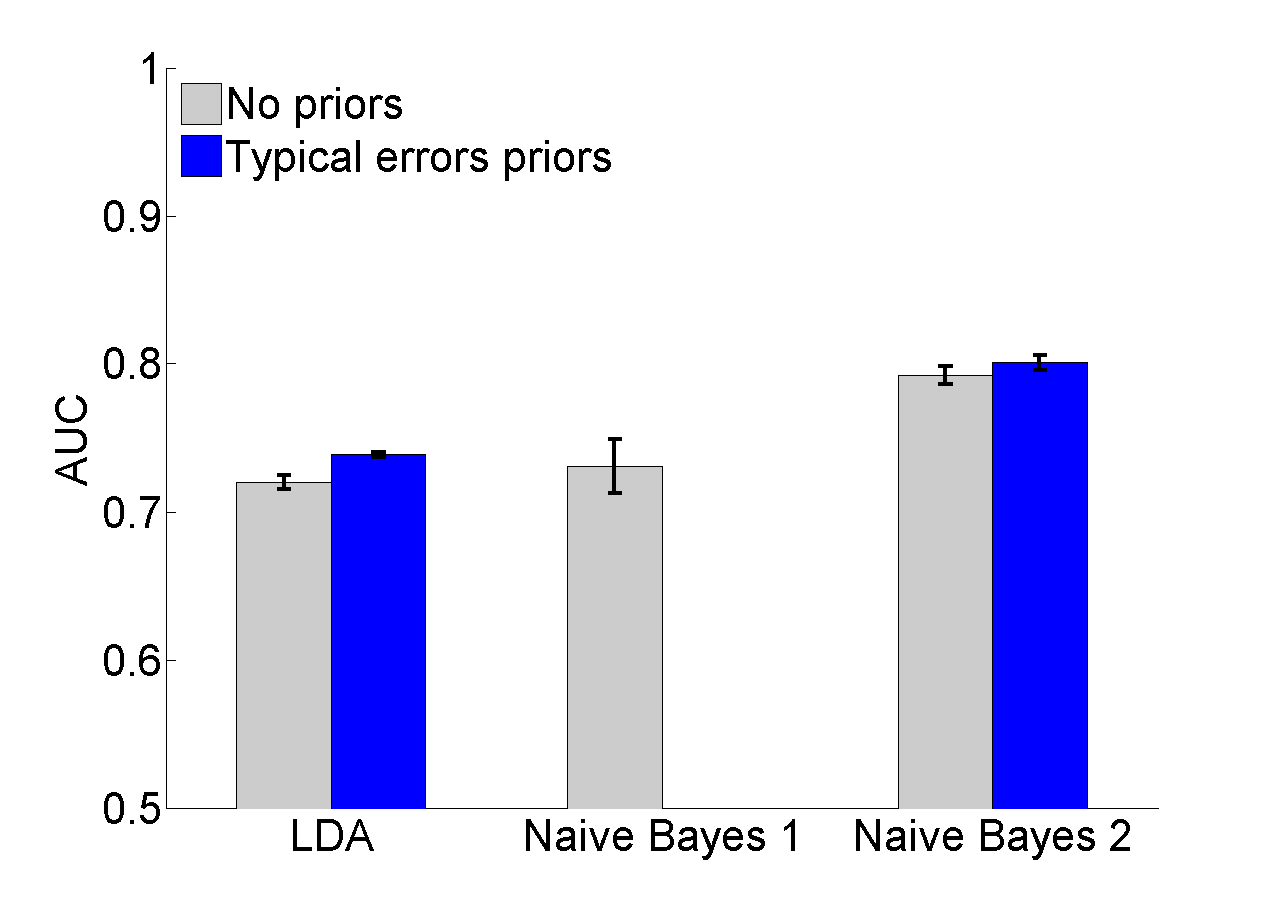
\includegraphics[width=\linewidth]{Figures/Ch1/AUC}
\caption{AUC values for the three graphical models – LDA, NB1 and NB2, with (dark bars) and without (light bars) typical errors priors to NB2 and LDA. Error bars denote the standard deviation over random splits of train and test subjects.}
\vspace{.3in}
\end{figure}

\begin{figure*}
\vspace{.3in}
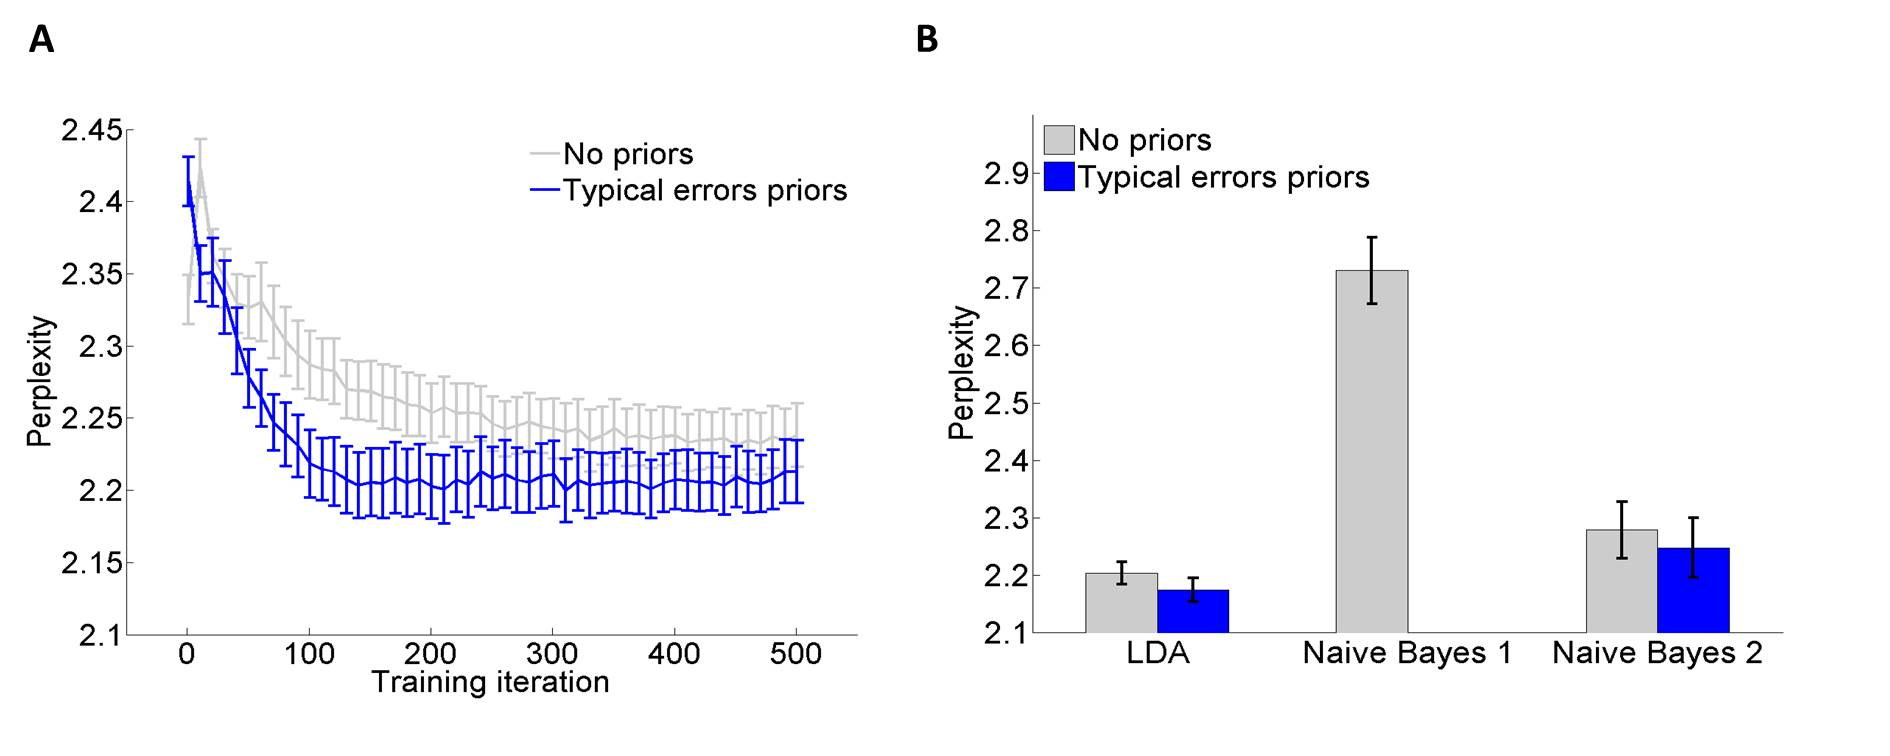
\includegraphics[width=\textwidth]{Figures/Ch1/figure5AB_HOZ}
\caption{(A) Perplexity values for the prediction set during training of the LDA model, with (dark curve) and without (light curve) typical-error priors. (B) A comparison between perplexity values calculated for the three models, with (dark bars) and without (light bars) typical-error priors to the NB2 and LDA models.}
\vspace{.3in}
\end{figure*}

 \vspace*{2\baselineskip}

Figure 1.3 shows the comparison between the accuracy of the models, table 1.2 summarizes the resulting AUC values. The highest accuracy is achieved with the NB2 model when it is provided with typical-errors priors $\beta_{wed}$. Next are the LDA when it is provided with typical-errors priors and the NB1 Models. Results reflect that the NB2 model is best at replicating diagnoses of experts, and therefore can be used as an automated data-driven tool for dyslexia diagnosis.

\begin{table}
\centering
\begin{tabular}{|c|c|c|c|} \hline
& NB1 & NB2 & LDA \\
\hline
&&&\\
Without & 0.731 & 0.792 & 0.720 \\
priors & (0.018) & (0.006) & (0.005) \\
&&&\\
\hline
&&&\\
With & --- & 0.801 & 0.739 \\
Priors &  & (0.005) & (0.002) \\
&&&\\
\hline\end{tabular}
\bigskip
\caption{AUC values for the three models. Standard deviation values over random split of train and test subjects are in parentheses.} 
\end{table}

As expected, the LDA model reasonably correlates with expert diagnosis. Yet, it predicts the same diagnosis as experts in fewer cases than NB2. In the following section we examine whether this is ought to the LDA model being an inaccurate model of dyslexia, or rather the opposite - it may contribute to expert knowledge in capturing dyslexic phenomena.

\subsection{The predictive power of the models}
Which model of the proposed models (NB1, NB2, LDA) best captures the hidden error patterns in the data, thereby best characterizing dyslexic errors? To answer this, we evaluate the predictive power of the three models using perplexity values over the prediction-set (figure 1.2).
The perplexity score is commonly used in assessing the predictive power of a language model (e.g., \citealp{bnj03}). It reflects the degree of "surprise" of the models to the errors made by the dyslexic person, and formally defined as: 

\begin{equation}
Perplexity = \exp{\Bigg(-\frac{\sum_{s=1}^{N_{test}} log(p(\bar{w_s}, \bar{e_s}))}{\sum_{s=1}^{N_{test}}|\bar{w_s}|}\Bigg)}.
\end{equation}

Here, it is evaluated on the prediction-set, where $ \bar{w_s} $ are the observed target-words and $ \bar{e_s} $ are the error types in the prediction-set of person p. $|\bar{w_s}|$ represents the number of words in the prediction-set ($|\bar{w_s}| = 98$), and $ N_{test} $ is the total number of test subjects ($ N_{test} = 219 $).

We also compare the predictive power of NB2 to LDA when provided with priors about the typical errors for each dyslexia subtype. Figure 1.4 shows that the perplexity of these two models is lower when provided with priors (figure 1.4: dark curve in panel A and dark bars in panel B). Incorporating expert knowledge into the model therefore increases its predictive power.

The prior value of the diagnosis distribution was set to be uniform with arbitrary value $ \alpha_{dp} = 0.05 $. The lower prior for the word-error-dyslexia distribution was set to $ \beta_{low} = 0.05 $, whereas for the higher prior $ \beta_{high} $, different values were explored. $ \beta_{high} $ is then chosen to be the value that achieves lowest perplexity $ \beta_{high} = 0.7 $ (figure 1.3). The perplexity values for all three models are summarized in figure 1.4b.

These results show that the best prediction of reading errors is achieved by the LDA model when it is provided with typical-errors priors (figure 1.4B). This result is consistent for different typical-error priors when compared to the NB2 model (figure 1.5). These results indicate that the LDA model best captures the hidden structure of reading errors, among all three models.

\begin{figure}[H]
\vspace{.3in}
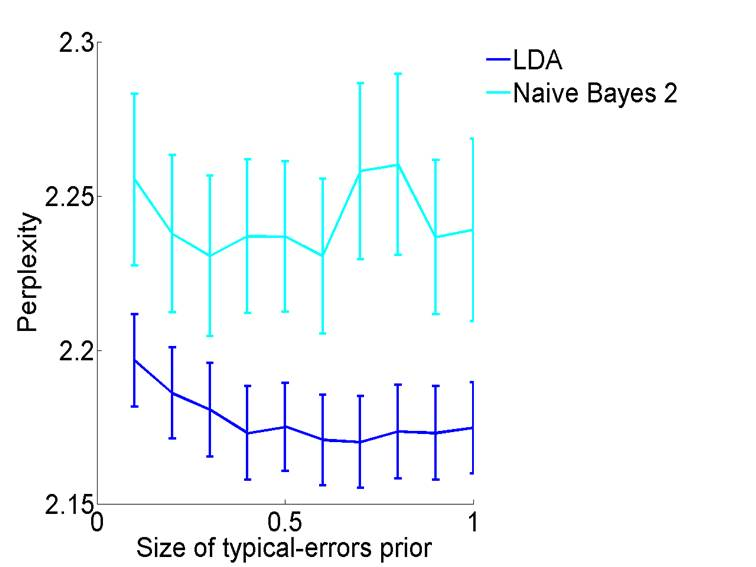
\includegraphics[width=\linewidth]{Figures/Ch1/figure5C.jpg}
\vspace{.3in}
\caption{Perplexity calculated for the NB2 and LDA models as a function of $\beta_{high}$, the size of the typical-error prior.}
\end{figure}

\subsection{The Dyslexia-Attention model of reading}
In addition to dyslexia, other factors may contribute to reading errors. For instance, people make reading mistakes due to momentarily lowered attention, which may be caused by an attention deficit or simply because they become tired as the diagnostic procedure progresses. These causes may interact with dyslexia. We hypothesized that we could "clean out" incorrect assignments of reading errors to dyslexia, rath\-er than to an unattended state, by disentangling errors caus\-ed by dyslexia from errors caused by low attention. We further hypothesized that by disentangling the two, we could classify between participants which are diagnosed with attention deficit disorder in addition to dyslexia. We therefore designed a model that takes into account the two possible causes of reading errors, specific dyslexia types and a generic low attention state, incorporating the manner in which these change during the diagnostic procedure. Specifically, we added to the LDA-based graphical model a binary random hidden variable marking the attentional state of the subject, attended or unattended, while reading each word. We set these attentional states as a hidden Markov chain, incorporating the dynamics of reading errors in time. We trained the model in a similar way to the LDA-based model, but this time also inferring the hidden attention states and learning the transition probabilities between these states.

When evaluating this model, following the same steps as in the above experiments, we did not find the Dyslexia-Attention model to improve over the dyslexia-state LDA model. We hypothesize that two reasons may explain the lack of improvement. First, adding the attention hidden variables requires a significantly larger number of parameters, which might be hard to well optimize with the current dataset. It is possible that training the model with an even larger corpus of data would improve the predictions. A second possible reason is that the attentional processes follow a different time scale than the one captured by the current experiments. The time spent in a state in an hidden Markov model follows an exponential distribution, and this may not be an adequate model for switching between attention states. 

\section{Discussion}
This study is a first demonstration of using probabilistic graphical models as a method for analyzing reading errors made by dyslexic people. The work has two main novel contributions: (a) it provides an automatic diagnosis tool of dyslexia, based on data of types of reading errors; (b) it provides probabilistic tools which enable exploring dyslexic phenomena based on reading errors data. By using these tools, the hidden structure of reading errors data, such as the probability of an error-type given a dyslexia and a target-word, may be extracted.

We tested three graphical models, a Latent Dirichlet Allocation (LDA) model and two Na\"{\i}ve-Bayes models, all differing by their complexity. The models were trained on a uniquely large data set of reading tests taken by dyslexic people.

Two experiments were conducted with the data to determine: (a) which model best captures the fine structure of the patterns of reading errors, and (b) which model best agrees with expert diagnoses. 

To answer the above questions, multiple models where train\-ed on a large corpus including 313 subjects and 196 target words in each test. Note that the majority of responses on the reading tests are correct responses of the subject, therefore most of the information about the structure of the errors resides in a small proportion of the data ($<20\%$). We expect accuracy of algorithms to improve as more data is accumulated.

The results show that the LDA model achieves best performance in terms of predicting reading errors, and it is therefore best in capturing the fine structure of the data. This result has both theoretical and practical implications. It may contribute to the understanding of dyslexic phenomena, and it may be used to improve designs of screening tests.

Another result of this study may serve as an application for diagnosis of dyslexia. NB2 was best in replicating diagnoses of experts ($AUC = 0.801$). This is yet another demonstration of Na\"{\i}ve-Bayes models being efficient classifiers. Note that in this study all models were trained on the screening-tests only, whereas diagnoses of clinicians are usually based on the results of the post-tests as well. The data-driven models, and particularly NB2, performed well in detecting the dyslexia subtype without leveraging the post-test information and thus are very effective.

Finally, the predictive power of the Na\"{\i}ve-Bayes and LDA models is improved when the models are provided with priors which are set according to knowledge of experts from the subtype approach. If the subtype approach were wrong, adding these priors would damage the predictive power of the model rather than improving it. The accuracy of these models is also improved when providing the models with such priors. Our work therefore provides support to the subtype approach to dyslexia, and exemplifies the ability of probabilistic graphical models to shed light on theoretical issues from different research fields, such as reading disorders in the case here.

The results of this study pave the way for clinical applications, such as using the algorithm of the NB2 model as a mobile application, providing an accessible and fast screening test, which allows people to obtain initial screening results, helping them decide whether further diagnosis is needed. This can be achieved by a mobile application which presents a series of words, asks the user to read them aloud, recognizes the spoken words, and uses the diagnosis algorithms described here to provide an initial diagnosis. The main challenge in achieving this is having the speech recognition component recognize utterances that are nonwords. Responses of dyslexic people may differ from existing words, whereas automatic speech recognizers (ASRs) are often trained to provide the most likely word elicited. For example, a subject may read an existing word such as \textit{cloud}, as another existing word \textit{could}, but also as a nonword such as \textit{clud}. This kind of distinction is crucial for the diagnosis. This challenge can be addressed by training and assessing ASR tools on data sets of labeled nonwords.

To conclude, this study is a demonstration of the use of probabilistic graphical models as a method of analyzing reading errors data. The progress presented in this chapter can also be deployed as a novel, efficient diagnostic tool for dyslexia, based on reading errors only. The Naive-Bayes model tested in this research was compared to labels given by experts in diagnosis of dyslexia, and was found to be an accurate and reliable candidate for an automated tool for initial screening of dyslexia, by its subtypes. 
